\documentclass[12pt]{article}

% --- Packages ---
\usepackage[utf8]{inputenc}
\usepackage{geometry}
\usepackage{amsmath, amssymb}
\usepackage{hyperref}
\usepackage{graphicx} % Required for \includegraphics
\usepackage{fancyhdr}
\usepackage{enumitem}
\usepackage{autobreak}
\usepackage{amsmath}
\usepackage{breqn}

\usepackage{amsmath,amssymb}
\usepackage{parskip}       % Correct paragraph spacing
\usepackage{xcolor}        % Required for \textcolor command
\usepackage{enumitem}
\usepackage{float}
\usepackage{listings}
\usepackage{xcolor}
\usepackage{tikz}
\usepackage[utf8]{inputenc}
\usepackage[T1]{fontenc}
\usepackage{url}
\usepackage{amsmath,amssymb,amsthm}
\usepackage{booktabs}
\usepackage{pgfplotstable}
\usepackage{siunitx}
\usepackage{geometry}
\usepackage[dvipsnames]{xcolor}
\newcommand{\T}[1]{\textcolor{ForestGreen}{#1}}
\newcommand{\F}[1]{\textcolor{red}{#1}}

\setlist{nosep}           % Reduce vertical spacing in lists
\usepackage{amsmath,amssymb}
\usepackage{geometry}
\usepackage{listings}
\usepackage{booktabs}
\usepackage{graphicx}
\usepackage{listings}
\usepackage{pgfplots}
\pgfplotsset{compat=1.18} % sau ultima versiune instalată la tine
\usepackage{filecontents} % dacă 
\setcounter{MaxMatrixCols}{12}
% --- Page Setup ---
\geometry{a4paper, margin=1in, top=1.2in, headheight=35pt} % Expanded top margin & headheight for the ornament

\lstset{
    language=python,
    basicstyle=\ttfamily\small,
    backgroundcolor=\color{blue!5},
    keywordstyle=\color{purple!80!blue},
    commentstyle=\color{green!50!black},
    stringstyle=\color{red!70!black},
    numberstyle=\tiny\color{gray},
    numbers=left,
    numbersep=15pt,
    frame=shadowbox,
    rulesepcolor=\color{blue!20},
    frameround=tttt,
    breaklines=true,
    captionpos=b,
    showstringspaces=false,
    tabsize=4,
    xleftmargin=20pt,
    xrightmargin=5pt
}

% --- Header & Footer Configuration ---
\pagestyle{fancy}
\fancyhf{} % Clear default headers/footers

% Center the ornament in the header (antet)
\chead{
\includegraphics[width=4cm]{../ornament_6.pdf}}

% Center the page number in the footer
\cfoot{\thepage}

% Optional: Remove the default rule line below the header
\renewcommand{\headrulewidth}{0pt}

\begin{document}

\begin{titlepage}
    \thispagestyle{fancy} % Force header/footer onto the title page
    \centering
    
    \vspace*{4cm}

    % Main Title
    {\Huge \bfseries Homework 5}

    \vspace{4cm}

    % Name and Date
    {\Large \textbf{Name:} Gatman Vitalie} \\[0.5em]
    {\Large \textbf{Date:} \today} \\[0.5em]
    {\Large \textbf{Group:} FAF-263}

    \vfill
\end{titlepage}

\newpage

% Page 2 content...
\section*{Problem 5.1}

Let $R$ be a relation on a nonempty set $X$. Is this relation reflexive, ireflexive, transitive, symmetric, antisymmetric, asymmetric, equivalence relation, weak/strong partial order, total order? If relation is an equivalence
relation, identify the equivalence classes.

\textcolor{red}{\rule{1em}{1em}} - No,    \textcolor{ForestGreen}{\rule{1em}{1em}} - Yes

% a) b) c)
\begin{enumerate}[label=\alph*)]
    \item \textcolor{ForestGreen}{Reflexive}, \textcolor{red}{Ireflexive}, \textcolor{ForestGreen}{Transitive}, \textcolor{ForestGreen}{Simetric}, \textcolor{red}{Antisimetric}, \textcolor{red}{Asymetric}, \textcolor{ForestGreen}{Equivalent},  \textcolor{red}{Weak}, \textcolor{red}{Strong}, \textcolor{red}{Total}, Classes: $\{1, 3, 5, 7, 9\}$ - even   $\{2, 4, 6, 8\}$ - odd
    \item \textcolor{Red}{Reflexive}, \textcolor{red}{Ireflexive}, \textcolor{red}{Transitive}, \textcolor{ForestGreen}{Simetric}, \textcolor{red}{Antisimetric}, \textcolor{red}{Asymetric}, \textcolor{red}{Equivalent},  \textcolor{red}{Weak}, \textcolor{red}{Strong}, \textcolor{red}{Total}.
    \item \textcolor{ForestGreen}{Reflexive}, \textcolor{Red}{Ireflexive}, \textcolor{ForestGreen}{Transitive}, \textcolor{ForestGreen}{Simetric}, \textcolor{red}{Antisimetric}, \textcolor{red}{Asymetric}, \textcolor{ForestGreen}{Equivalent},  \textcolor{red}{Weak}, \textcolor{red}{Strong}, \textcolor{red}{Total}, $  [(a,b)] = \{ (x,y)\in\mathbb{R}^2 \mid x^2+y^2 = a^2+b^2 \}.$
    \item\F{Reflexive}, \T{Irreflexive}, \F{Transitive}, \T{Symmetric}, \F{Antisymmetric}, \F{Asymmetric}, \F{Equivalence}, \F{Weak}, \F{Strong}, \F{Total}.
    \item \F{Reflexive}, \T{Irreflexive}, \T{Transitive}, \F{Symmetric}, \T{Antisymmetric}, \T{Asymmetric}, \F{Equivalence}, \F{Weak}, \T{Strong}, \F{Total}.
    \item \F{Reflexive}, \T{Irreflexive}, \T{Transitive}, \F{Symmetric}, \T{Antisymmetric}, \T{Asymmetric}, \F{Equivalence}, \F{Weak}, \T{Strong}, \F{Total}.
    \item \T{Reflexive}, \F{Irreflexive}, \T{Transitive}, \F{Symmetric}, \T{Antisymmetric}, \F{Asymmetric}, \F{Equivalence}, \T{Weak}, \F{Strong}, \T{Total}.
    \item \T{Reflexive}, \F{Irreflexive}, \T{Transitive}, \F{Symmetric}, \T{Antisymmetric}, \F{Asymmetric}, \F{Equivalence}, \T{Weak}, \F{Strong}, \F{Total}.
\end{enumerate}
\section*{Problem 5.2}
\begin{enumerate}[label=\alph*)]
  \item Beceuse the first diagonal is full, i mean has only 1 them $M_R$ is refelxive and clery not irefelxible. $M_R^T \not= M_R$ so R is not symetric. Because we proved that R is refelxive it cann't be asymetric. It is olso antisimetric because because if we check the simetry relative to the first diagonal we do not see a pair of pairs wich are both 1. \[M_R^2=\begin{pmatrix}
1 & 1 & 1 & 1 \\
0 & 1 & 0 & 1 \\
0 & 0 & 1 & 1 \\
0 & 0 & 0 & 1
\end{pmatrix}\] 
and we can crlery see that $M_R^2=M_R$ so R is transitive.\\
    So R in a partial weak order.
\item  \noindent
\begin{center}
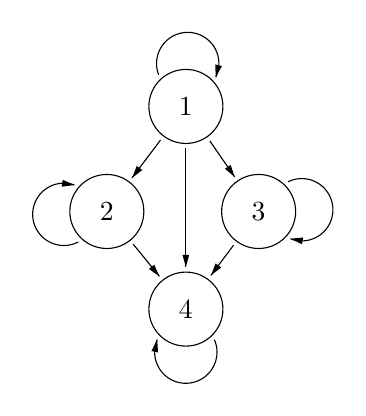
\begin{tikzpicture}[scale=0.2]
\draw (56.71, -9.33) circle (2.35);
\draw (56.71, -9.33) node {\normalsize $1$};
\draw (51.69, -16.00) circle (2.35);
\draw (51.69, -16.00) node {\normalsize $2$};
\draw (61.33, -16.00) circle (2.35);
\draw (61.33, -16.00) node {\normalsize $3$};
\draw (56.71, -22.20) circle (2.35);
\draw (56.71, -22.20) node {\normalsize $4$};
\draw (55.10, -11.46) -- (53.29, -13.87);
\fill (53.59,-13.11) -- (53.94,-13.37) -- (53.29,-13.87) -- cycle;
\draw (58.23, -11.52) -- (59.81, -13.81);
\fill (59.19,-13.29) -- (59.55,-13.04) -- (59.81,-13.81) -- cycle;
\draw (56.71, -12.00) -- (56.71, -19.53);
\fill (56.49,-18.75) -- (56.92,-18.75) -- (56.71,-19.53) -- cycle;
\draw (53.36, -18.07) -- (55.03, -20.12);
\fill (54.36,-19.65) -- (54.70,-19.38) -- (55.03,-20.12) -- cycle;
\draw (59.74, -18.14) -- (58.30, -20.06);
\fill (58.60,-19.30) -- (58.95,-19.56) -- (58.30,-20.06) -- cycle;
\draw (54.98, -7.32) arc (-158.8327:-385.9392:1.98);
\fill (58.58,-6.66) -- (59.00,-6.77) -- (58.60,-7.47) -- cycle;
\draw (63.20, -14.11) arc (115.9392:-111.1673:1.98);
\fill (64.16,-17.65) -- (64.08,-18.08) -- (63.35,-17.73) -- cycle;
\draw (49.87, -17.94) arc (-62.6326:-289.7392:1.98);
\fill (48.82,-14.43) -- (48.89,-13.99) -- (49.63,-14.32) -- cycle;
\draw (58.52, -24.14) arc (23.5533:-203.5533:1.98);
\fill (54.94,-24.95) -- (54.52,-24.86) -- (54.89,-24.14) -- cycle;
\end{tikzpicture}
\end{center}
\item The minimal is 1 because no other nods besides itself goes into it and the maximum is 4 beceause all nodes goo into it and there it does exist other vertext with that properti 
\end{enumerate}

\section*{Problem 5.3}
%a) b) c)
\begin{enumerate}[label=\alph*)]
    \item Yes because $R^{-1} = { (b, a) : (a, b) \in R }$ so if a relation is antisymmtric if has the property that $(a\sim b) \land (b\sim a) \implies a=b $ but because $and$ and $=$ is comunative them olso $(b\sim a) \land (a\sim b) \implies a=b$ wich is the same as writin g$R^{-1}$ is antisimetric
    \item $R^{-1} = { (b, a) : (a, b) \in R }$. Yes because if $R$ is simetric them $(a \sim b) \implies (b \sim a)$ but if $R=R^{-1}$ them that means that for evry pair $(a \sim b)$ in $R$ exist olso in $R^{-1}$ and evry pair $(b \sim a)$ in $R^{-1}$ olso exist in $R^{-1}$ wich just proves that the existe of one pair proves the invers wich indit is simetry.
    \item If $R$ is transitive that means that for some aribtrary set $(a\sim c)$ there exist $(a\sim b)$ and $(b\sim c)$ where $(a\sim b)$ and $(b\sim c)$ are in $R$  and now lest looks what $R \circ R$ is. $R \circ R = { (a, c) : \exists b \in X, (a, b) \in R \land (b, c) \in R }$ so if we take $(a\sim b)$ and $(b\sim c)$ from $R$ we can see that $(a\sim c)$ is in $R \circ R$ but because $R$ is transitive that means that $(a\sim c)$ is in $R$ so we can conclude that $R \circ R \subseteq R$
\end{enumerate}

\section*{Problem 5.4}
\begin{enumerate}[label=\alph*)]
\item 
\[
M_{\#}=\begin{pmatrix}
1 & 0 & 0 & 0 & 0 & 0 & 0 & 0 & 0 & 0 & 0 & 0\\
1 & 1 & 0 & 0 & 0 & 0 & 0 & 0 & 0 & 0 & 0 & 0\\
1 & 0 & 1 & 0 & 0 & 0 & 0 & 0 & 0 & 0 & 0 & 0\\
1 & 1 & 0 & 1 & 0 & 0 & 0 & 0 & 0 & 0 & 0 & 0\\
1 & 0 & 0 & 0 & 1 & 0 & 0 & 0 & 0 & 0 & 0 & 0\\
1 & 1 & 1 & 0 & 0 & 1 & 0 & 0 & 0 & 0 & 0 & 0\\
1 & 0 & 0 & 0 & 0 & 0 & 1 & 0 & 0 & 0 & 0 & 0\\
1 & 1 & 0 & 1 & 0 & 0 & 0 & 1 & 0 & 0 & 0 & 0\\
1 & 0 & 1 & 0 & 0 & 0 & 0 & 0 & 1 & 0 & 0 & 0\\
1 & 1 & 0 & 0 & 1 & 0 & 0 & 0 & 0 & 1 & 0 & 0\\
1 & 0 & 0 & 0 & 0 & 0 & 0 & 0 & 0 & 0 & 1 & 0\\
1 & 1 & 1 & 1 & 0 & 1 & 0 & 0 & 0 & 0 & 0 & 1
\end{pmatrix}.
\]
\item \noindent 
\begin{center}
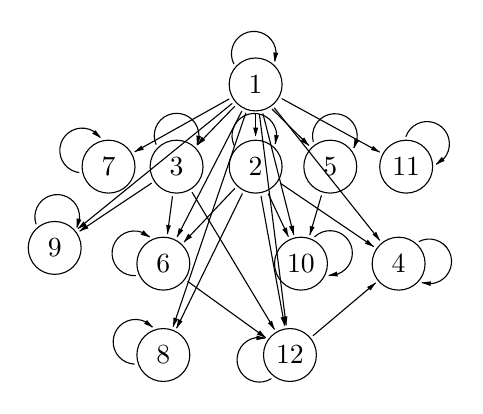
\begin{tikzpicture}[scale = 0.4]
\draw (19.22, -3.45) circle (0.84);
\draw (19.22, -3.45) node {\normalsize $1$};
\draw (19.22, -6.06) circle (0.84);
\draw (19.22, -6.06) node {\normalsize $2$};
\draw (16.71, -6.06) circle (0.84);
\draw (16.71, -6.06) node {\normalsize $3$};
\draw (23.76, -9.14) circle (0.84);
\draw (23.76, -9.14) node {\normalsize $4$};
\draw (21.59, -6.06) circle (0.84);
\draw (21.59, -6.06) node {\normalsize $5$};
\draw (16.29, -9.14) circle (0.84);
\draw (16.29, -9.14) node {\normalsize $6$};
\draw (14.55, -6.06) circle (0.84);
\draw (14.55, -6.06) node {\normalsize $7$};
\draw (16.29, -12.04) circle (0.84);
\draw (16.29, -12.04) node {\normalsize $8$};
\draw (12.84, -8.64) circle (0.84);
\draw (12.84, -8.64) node {\normalsize $9$};
\draw (20.66, -9.14) circle (0.84);
\draw (20.66, -9.14) node {\normalsize $10$};
\draw (24.00, -6.06) circle (0.84);
\draw (24.00, -6.06) node {\normalsize $11$};
\draw (20.31, -12.04) circle (0.84);
\draw (20.31, -12.04) node {\normalsize $12$};
\draw (13.62, -6.25) arc (-97.4105:-324.5170:0.71);
\fill (14.03,-5.01) -- (14.14,-4.90) -- (14.29,-5.14) -- cycle;
\draw (18.38, -3.91) -- (15.38, -5.59);
\fill (15.59,-5.39) -- (15.67,-5.52) -- (15.38,-5.59) -- cycle;
\draw (18.53, -2.80) arc (-152.8055:-379.9120:0.71);
\fill (19.78,-2.43) -- (19.94,-2.45) -- (19.82,-2.72) -- cycle;
\draw (18.56, -4.14) -- (17.37, -5.37);
\fill (17.51,-5.11) -- (17.62,-5.22) -- (17.37,-5.37) -- cycle;
\draw (19.22, -4.40) -- (19.22, -5.10);
\fill (19.14,-4.82) -- (19.30,-4.82) -- (19.22,-5.10) -- cycle;
\draw (19.74, -4.23) -- (20.91, -5.39);
\fill (20.65,-5.25) -- (20.76,-5.13) -- (20.91,-5.39) -- cycle;
\draw (20.05, -3.90) -- (23.16, -5.60);
\fill (22.88,-5.53) -- (22.95,-5.40) -- (23.16,-5.60) -- cycle;
\draw (16.06, -5.36) arc (-156.4467:-383.5533:0.71);
\fill (17.34,-5.07) -- (17.49,-5.10) -- (17.36,-5.36) -- cycle;
\draw (18.54, -5.39) arc (-154.1560:-381.2625:0.71);
\fill (19.81,-5.05) -- (19.96,-5.07) -- (19.84,-5.34) -- cycle;
\draw (21.05, -5.27) arc (-165.1929:-392.2995:0.71);
\fill (22.36,-5.18) -- (22.51,-5.23) -- (22.33,-5.47) -- cycle;
\draw (23.99, -5.11) arc (161.2796:-65.8270:0.71);
\fill (25.13,-5.75) -- (25.22,-5.88) -- (24.95,-5.98) -- cycle;
\draw (18.56, -6.75) -- (16.95, -8.45);
\fill (17.08,-8.19) -- (17.20,-8.30) -- (16.95,-8.45) -- cycle;
\draw (16.58, -7.00) -- (16.42, -8.20);
\fill (16.38,-7.91) -- (16.53,-7.93) -- (16.42,-8.20) -- cycle;
\draw (15.92, -6.58) -- (13.63, -8.11);
\fill (13.82,-7.89) -- (13.91,-8.02) -- (13.63,-8.11) -- cycle;
\draw (19.39, -6.99) -- (20.14, -11.11);
\fill (20.01,-10.85) -- (20.17,-10.82) -- (20.14,-11.11) -- cycle;
\draw (21.04, -11.43) -- (23.03, -9.75);
\fill (22.87,-9.99) -- (22.76,-9.88) -- (23.03,-9.75) -- cycle;
\draw (17.20, -6.87) -- (19.82, -11.23);
\fill (19.61,-11.03) -- (19.74,-10.95) -- (19.82,-11.23) -- cycle;
\draw (12.25, -7.89) arc (-160.8454:-387.9520:0.71);
\fill (13.54,-7.70) -- (13.69,-7.75) -- (13.54,-7.99) -- cycle;
\draw (15.42, -9.52) arc (-86.1005:-313.2071:0.71);
\fill (15.57,-8.22) -- (15.66,-8.08) -- (15.85,-8.30) -- cycle;
\draw (21.09, -8.29) arc (133.7781:-93.3284:0.71);
\fill (21.80,-9.39) -- (21.83,-9.55) -- (21.54,-9.51) -- cycle;
\draw (24.40, -8.44) arc (117.7587:-109.3479:0.71);
\fill (24.79,-9.70) -- (24.77,-9.85) -- (24.50,-9.74) -- cycle;
\draw (19.62, -6.92) -- (20.26, -8.28);
\fill (20.07,-8.06) -- (20.21,-7.99) -- (20.26,-8.28) -- cycle;
\draw (21.31, -6.97) -- (20.94, -8.23);
\fill (20.94,-7.94) -- (21.09,-7.98) -- (20.94,-8.23) -- cycle;
\draw (20.01, -6.59) -- (22.97, -8.60);
\fill (22.69,-8.51) -- (22.78,-8.38) -- (22.97,-8.60) -- cycle;
\draw (18.80, -6.91) -- (16.71, -11.19);
\fill (16.76,-10.90) -- (16.90,-10.97) -- (16.71,-11.19) -- cycle;
\draw (15.38, -12.33) arc (-92.1723:-319.2789:0.71);
\fill (15.68,-11.05) -- (15.77,-10.93) -- (15.95,-11.16) -- cycle;
\draw (19.72, -12.79) arc (-57.6049:-284.7115:0.71);
\fill (19.24,-11.57) -- (19.25,-11.42) -- (19.53,-11.51) -- cycle;
\draw (17.06, -9.70) -- (19.54, -11.49);
\fill (19.26,-11.39) -- (19.36,-11.26) -- (19.54,-11.49) -- cycle;
\draw (18.48, -4.05) -- (13.58, -8.03);
\fill (13.75,-7.80) -- (13.85,-7.92) -- (13.58,-8.03) -- cycle;
\draw (18.78, -4.30) -- (16.73, -8.29);
\fill (16.78,-8.01) -- (16.92,-8.08) -- (16.73,-8.29) -- cycle;
\draw (19.45, -4.37) -- (20.43, -8.22);
\fill (20.28,-7.96) -- (20.44,-7.93) -- (20.43,-8.22) -- cycle;
\draw (19.81, -4.19) -- (23.16, -8.40);
\fill (22.93,-8.22) -- (23.05,-8.13) -- (23.16,-8.40) -- cycle;
\draw (19.34, -4.39) -- (20.19, -11.10);
\fill (20.08,-10.83) -- (20.23,-10.81) -- (20.19,-11.10) -- cycle;
\draw (18.91, -4.35) -- (16.60, -11.14);
\fill (16.61,-10.85) -- (16.76,-10.90) -- (16.60,-11.14) -- cycle;
\end{tikzpicture}
\end{center}
\item \noindent 
\begin{center}
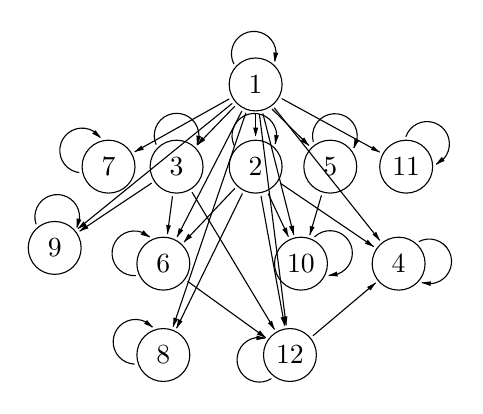
\begin{tikzpicture}[scale = 0.4]
\draw (19.22, -3.45) circle (0.84);
\draw (19.22, -3.45) node {\normalsize $1$};
\draw (19.22, -6.06) circle (0.84);
\draw (19.22, -6.06) node {\normalsize $2$};
\draw (16.71, -6.06) circle (0.84);
\draw (16.71, -6.06) node {\normalsize $3$};
\draw (23.76, -9.14) circle (0.84);
\draw (23.76, -9.14) node {\normalsize $4$};
\draw (21.59, -6.06) circle (0.84);
\draw (21.59, -6.06) node {\normalsize $5$};
\draw (16.29, -9.14) circle (0.84);
\draw (16.29, -9.14) node {\normalsize $6$};
\draw (14.55, -6.06) circle (0.84);
\draw (14.55, -6.06) node {\normalsize $7$};
\draw (16.29, -12.04) circle (0.84);
\draw (16.29, -12.04) node {\normalsize $8$};
\draw (12.84, -8.64) circle (0.84);
\draw (12.84, -8.64) node {\normalsize $9$};
\draw (20.66, -9.14) circle (0.84);
\draw (20.66, -9.14) node {\normalsize $10$};
\draw (24.00, -6.06) circle (0.84);
\draw (24.00, -6.06) node {\normalsize $11$};
\draw (20.31, -12.04) circle (0.84);
\draw (20.31, -12.04) node {\normalsize $12$};
\draw (13.62, -6.25) arc (-97.4105:-324.5170:0.71);
\fill (14.03,-5.01) -- (14.14,-4.90) -- (14.29,-5.14) -- cycle;
\draw (18.38, -3.91) -- (15.38, -5.59);
\fill (15.59,-5.39) -- (15.67,-5.52) -- (15.38,-5.59) -- cycle;
\draw (18.53, -2.80) arc (-152.8055:-379.9120:0.71);
\fill (19.78,-2.43) -- (19.94,-2.45) -- (19.82,-2.72) -- cycle;
\draw (18.56, -4.14) -- (17.37, -5.37);
\fill (17.51,-5.11) -- (17.62,-5.22) -- (17.37,-5.37) -- cycle;
\draw (19.22, -4.40) -- (19.22, -5.10);
\fill (19.14,-4.82) -- (19.30,-4.82) -- (19.22,-5.10) -- cycle;
\draw (19.74, -4.23) -- (20.91, -5.39);
\fill (20.65,-5.25) -- (20.76,-5.13) -- (20.91,-5.39) -- cycle;
\draw (20.05, -3.90) -- (23.16, -5.60);
\fill (22.88,-5.53) -- (22.95,-5.40) -- (23.16,-5.60) -- cycle;
\draw (16.06, -5.36) arc (-156.4467:-383.5533:0.71);
\fill (17.34,-5.07) -- (17.49,-5.10) -- (17.36,-5.36) -- cycle;
\draw (18.54, -5.39) arc (-154.1560:-381.2625:0.71);
\fill (19.81,-5.05) -- (19.96,-5.07) -- (19.84,-5.34) -- cycle;
\draw (21.05, -5.27) arc (-165.1929:-392.2995:0.71);
\fill (22.36,-5.18) -- (22.51,-5.23) -- (22.33,-5.47) -- cycle;
\draw (23.99, -5.11) arc (161.2796:-65.8270:0.71);
\fill (25.13,-5.75) -- (25.22,-5.88) -- (24.95,-5.98) -- cycle;
\draw (18.56, -6.75) -- (16.95, -8.45);
\fill (17.08,-8.19) -- (17.20,-8.30) -- (16.95,-8.45) -- cycle;
\draw (16.58, -7.00) -- (16.42, -8.20);
\fill (16.38,-7.91) -- (16.53,-7.93) -- (16.42,-8.20) -- cycle;
\draw (15.92, -6.58) -- (13.63, -8.11);
\fill (13.82,-7.89) -- (13.91,-8.02) -- (13.63,-8.11) -- cycle;
\draw (19.39, -6.99) -- (20.14, -11.11);
\fill (20.01,-10.85) -- (20.17,-10.82) -- (20.14,-11.11) -- cycle;
\draw (21.04, -11.43) -- (23.03, -9.75);
\fill (22.87,-9.99) -- (22.76,-9.88) -- (23.03,-9.75) -- cycle;
\draw (17.20, -6.87) -- (19.82, -11.23);
\fill (19.61,-11.03) -- (19.74,-10.95) -- (19.82,-11.23) -- cycle;
\draw (12.25, -7.89) arc (-160.8454:-387.9520:0.71);
\fill (13.54,-7.70) -- (13.69,-7.75) -- (13.54,-7.99) -- cycle;
\draw (15.42, -9.52) arc (-86.1005:-313.2071:0.71);
\fill (15.57,-8.22) -- (15.66,-8.08) -- (15.85,-8.30) -- cycle;
\draw (21.09, -8.29) arc (133.7781:-93.3284:0.71);
\fill (21.80,-9.39) -- (21.83,-9.55) -- (21.54,-9.51) -- cycle;
\draw (24.40, -8.44) arc (117.7587:-109.3479:0.71);
\fill (24.79,-9.70) -- (24.77,-9.85) -- (24.50,-9.74) -- cycle;
\draw (19.62, -6.92) -- (20.26, -8.28);
\fill (20.07,-8.06) -- (20.21,-7.99) -- (20.26,-8.28) -- cycle;
\draw (21.31, -6.97) -- (20.94, -8.23);
\fill (20.94,-7.94) -- (21.09,-7.98) -- (20.94,-8.23) -- cycle;
\draw (20.01, -6.59) -- (22.97, -8.60);
\fill (22.69,-8.51) -- (22.78,-8.38) -- (22.97,-8.60) -- cycle;
\draw (18.80, -6.91) -- (16.71, -11.19);
\fill (16.76,-10.90) -- (16.90,-10.97) -- (16.71,-11.19) -- cycle;
\draw (15.38, -12.33) arc (-92.1723:-319.2789:0.71);
\fill (15.68,-11.05) -- (15.77,-10.93) -- (15.95,-11.16) -- cycle;
\draw (19.72, -12.79) arc (-57.6049:-284.7115:0.71);
\fill (19.24,-11.57) -- (19.25,-11.42) -- (19.53,-11.51) -- cycle;
\draw (17.06, -9.70) -- (19.54, -11.49);
\fill (19.26,-11.39) -- (19.36,-11.26) -- (19.54,-11.49) -- cycle;
\draw (18.48, -4.05) -- (13.58, -8.03);
\fill (13.75,-7.80) -- (13.85,-7.92) -- (13.58,-8.03) -- cycle;
\draw (18.78, -4.30) -- (16.73, -8.29);
\fill (16.78,-8.01) -- (16.92,-8.08) -- (16.73,-8.29) -- cycle;
\draw (19.45, -4.37) -- (20.43, -8.22);
\fill (20.28,-7.96) -- (20.44,-7.93) -- (20.43,-8.22) -- cycle;
\draw (19.81, -4.19) -- (23.16, -8.40);
\fill (22.93,-8.22) -- (23.05,-8.13) -- (23.16,-8.40) -- cycle;
\draw (19.34, -4.39) -- (20.19, -11.10);
\fill (20.08,-10.83) -- (20.23,-10.81) -- (20.19,-11.10) -- cycle;
\draw (18.91, -4.35) -- (16.60, -11.14);
\fill (16.61,-10.85) -- (16.76,-10.90) -- (16.60,-11.14) -- cycle;
\end{tikzpicture}
\end{center}
\item Reflexive: for every $x\in A$, $x=1\cdot x$, so $x\,\#\,x$.

Antisymmetric: we have a pair $x\,\#\,y$ and $y\,\#\,x$. Then $x=ky$ and $y=mx$ for some
$k\sim m\in\mathbb{N}^{+}$, because $x=kmx$, we get $km=1$. We knoe that $k\sim m$ are positive integers,
$k=m=1$ and therefore $x=y$.

Transitive: we have the relation properties $x\,\#\,y$ and $y\,\#\,z$. Therefore $x=ky$ and $y=mz$, so
$x=(km)z$ with $km\in\mathbb{N}^{+}$. Hence $x\,\#\,z$.
Therefore $\#$ is reflexive, antisymmetric and transitive, so it is a (weak) partial order on $A$.
\item $\#$ is not a total order because $2$ and $3$ are incomparable.
\end{enumerate}

% TO chech tomorow
\section*{Problem 5.5}
\begin{enumerate}[label=\alph*)]
    \item Let $R=\{(a,a)\mid a\in A\}$, i.e.\ $a\,R\,b \iff a=b$.
$R$ is reflexive, since $(a,a)\in R$ for all $a$.
$R$ is symmetric, since $a=b$ implies $b=a$.
$R$ is antisymmetric, since $aRb$ and $bRa$ give $a=b$ directly.
$R$ is transitive, since $a=b$ and $b=c$ imply $a=c$.
Hence $R$ is both an equivalence relation and a (weak) partial order on $A$.
In fact it is the only such relation: if $R$ is symmetric and antisymmetric,
any pair $(a,b)\in R$ must satisfy $a=b$, and reflexivity then forces $R$ to
contain all pairs $(a,a)$.
\item $R$ is a total order only when $|A|=1$. If $|A|\ge 2$, take $a\neq b$ in $A$:
then $(a,b)\notin R$ and $(b,a)\notin R$, so $a$ and $b$ are incomparable and $R$ is not total.
\end{enumerate}

\section*{Problem 5.6}
\begin{enumerate}[label=\alph*)]
    \item $A\rightarrow D \rightarrow E \rightarrow G$
    \item $\{A, B, C\}$ $\{A, B, D\}$
    \item it is determinated by the longest chain size wich is in point a) and its size is 4
    \item We do this way $\{A, B\} \rightarrow \{D, C\} \rightarrow \{E, F\} \rightarrow \{G, H\}$ so the asnwe is $t=4$
\end{enumerate}

\section*{Problem 5.7}
\begin{enumerate}[label=\alph*)]
    \item It is a poset. By the definition $x=y$ it is reflexive, and $x$ mut be done beofre $y$ for all $x$ and  in $(S, \preccurlyeq)$ thus is olso transitive. For it to be clasified as a posed it should be antisimetric wich it clery is because is trantitive and there does not exist a closed loop wich we can prove by manualy folowing the tasks.
   \newpage \item \noindent



\begin{center}
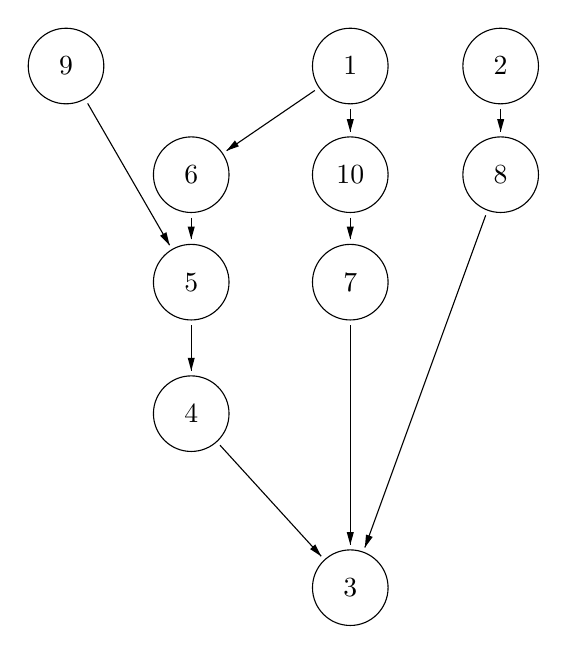
\begin{tikzpicture}[scale=0.5]
\draw (24.29, -1.12) circle (0.96);
\draw (24.29, -1.12) node {\normalsize $1$};
\draw (20.25, -3.88) circle (0.96);
\draw (20.25, -3.88) node { $6$};
\draw (24.29, -3.88) circle (0.96);
\draw (24.29, -3.88) node { $10$};
\draw (28.11, -1.12) circle (0.96);
\draw (28.11, -1.12) node { $2$};
\draw (28.11, -3.88) circle (0.96);
\draw (28.11, -3.88) node { $8$};
\draw (20.25, -9.95) circle (0.96);
\draw (20.25, -9.95) node { $4$};
\draw (20.25, -6.61) circle (0.96);
\draw (20.25, -6.61) node { $5$};
\draw (24.29, -6.61) circle (0.96);
\draw (24.29, -6.61) node { $7$};
\draw (24.29, -14.37) circle (0.96);
\draw (24.29, -14.37) node { $3$};
\draw (17.07, -1.12) circle (0.96);
\draw (17.07, -1.12) node { $9$};
\draw (23.39, -1.74) -- (21.15, -3.27);
\fill (21.36,-3.01) -- (21.46,-3.16) -- (21.15,-3.27) -- cycle;
\draw (24.29, -2.21) -- (24.29, -2.79);
\fill (24.20,-2.47) -- (24.38,-2.47) -- (24.29,-2.79) -- cycle;
\draw (28.11, -2.21) -- (28.11, -2.79);
\fill (28.02,-2.47) -- (28.20,-2.47) -- (28.11,-2.79) -- cycle;
\draw (20.25, -7.70) -- (20.25, -8.86);
\fill (20.16,-8.53) -- (20.34,-8.53) -- (20.25,-8.86) -- cycle;
\draw (20.25, -4.97) -- (20.25, -5.52);
\fill (20.16,-5.20) -- (20.34,-5.20) -- (20.25,-5.52) -- cycle;
\draw (24.29, -7.70) -- (24.29, -13.28);
\fill (24.20,-12.96) -- (24.38,-12.96) -- (24.29,-13.28) -- cycle;
\draw (27.73, -4.91) -- (24.66, -13.35);
\fill (24.69,-13.02) -- (24.86,-13.08) -- (24.66,-13.35) -- cycle;
\draw (17.62, -2.07) -- (19.70, -5.67);
\fill (19.46,-5.43) -- (19.62,-5.34) -- (19.70,-5.67) -- cycle;
\draw (20.98, -10.75) -- (23.55, -13.57);
\fill (23.27,-13.39) -- (23.40,-13.27) -- (23.55,-13.57) -- cycle;
\draw (24.29, -4.97) -- (24.29, -5.52);
\fill (24.20,-5.20) -- (24.38,-5.20) -- (24.29,-5.52) -- cycle;
\end{tikzpicture}
\end{center}
    \item Minimal emenetra are $\{1, 2, 9\}$ the maximal elemen is $3$, longest chain is \\ $1 \rightarrow 6 \rightarrow 5 \rightarrow 4 \rightarrow 3$ and longest antichain $\{9, 6, 10, 8\}$
    \item A posible sort is $9\rightarrow 1\rightarrow 2 \rightarrow 6 \rightarrow 10 \rightarrow 8 \rightarrow 5 \rightarrow 7 \rightarrow 4 \rightarrow 5$ but we just need to clearr all element of a layers so there are other methods to do the tasks.
    \item From a) the longest chain has a size of 5 so the answer is $t=5$
\end{enumerate}

\section*{Problem 5.8}
\begin{enumerate}[label=\alph*)]
    \item \noindent
    \begin{center}
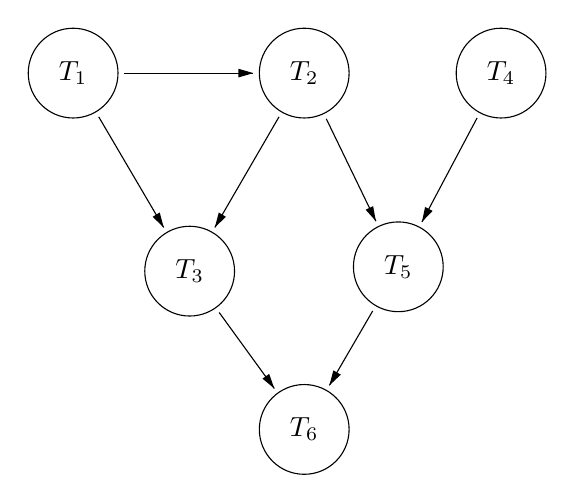
\begin{tikzpicture}[scale=0.5]
\draw (25.93, -12.23) circle (1.14);
\draw (25.93, -12.23) node { $T_6$};
\draw (23.02, -8.21) circle (1.14);
\draw (23.02, -8.21) node { $T_3$};
\draw (28.32, -8.10) circle (1.14);
\draw (28.32, -8.10) node { $T_5$};
\draw (20.06, -3.18) circle (1.14);
\draw (20.06, -3.18) node { $T_1$};
\draw (25.93, -3.18) circle (1.14);
\draw (25.93, -3.18) node { $T_2$};
\draw (30.93, -3.18) circle (1.14);
\draw (30.93, -3.18) node { $T_4$};
\draw (20.71, -4.29) -- (22.36, -7.10);
\fill (22.08,-6.83) -- (22.26,-6.72) -- (22.36,-7.10) -- cycle;
\draw (25.29, -4.29) -- (23.66, -7.10);
\fill (23.76,-6.72) -- (23.94,-6.83) -- (23.66,-7.10) -- cycle;
\draw (23.77, -9.26) -- (25.17, -11.19);
\fill (24.87,-10.94) -- (25.04,-10.82) -- (25.17,-11.19) -- cycle;
\draw (27.67, -9.22) -- (26.57, -11.11);
\fill (26.67,-10.73) -- (26.86,-10.84) -- (26.57,-11.11) -- cycle;
\draw (26.49, -4.34) -- (27.75, -6.94);
\fill (27.49,-6.65) -- (27.68,-6.56) -- (27.75,-6.94) -- cycle;
\draw (30.32, -4.32) -- (28.92, -6.96);
\fill (29.00,-6.58) -- (29.19,-6.68) -- (28.92,-6.96) -- cycle;
\draw (21.35, -3.18) -- (24.64, -3.18);
\fill (24.26,-3.29) -- (24.26,-3.07) -- (24.64,-3.18) -- cycle;
\end{tikzpicture}
\end{center}
\item Is posible. From the DAG we can see that there aren't any closed loops. We can do this way $T_1 \rightarrow T_2 \rightarrow T_4 \rightarrow T_3 \rightarrow T_5 \rightarrow T_6$ and we can see that all tasks are done, and this is just one posible configuartion as long as we cleared the previsousle layers the order does not matter.
\item The longest chain is $T_1 \rightarrow T_2 \rightarrow T_3 \rightarrow T_6$ and its size is 4, so the answer is $t=4$
\end{enumerate}
\newpage
\section*{Problem 5.9}
\begin{enumerate}[label=\alph*)]
    \item \noindent
    \begin{center}
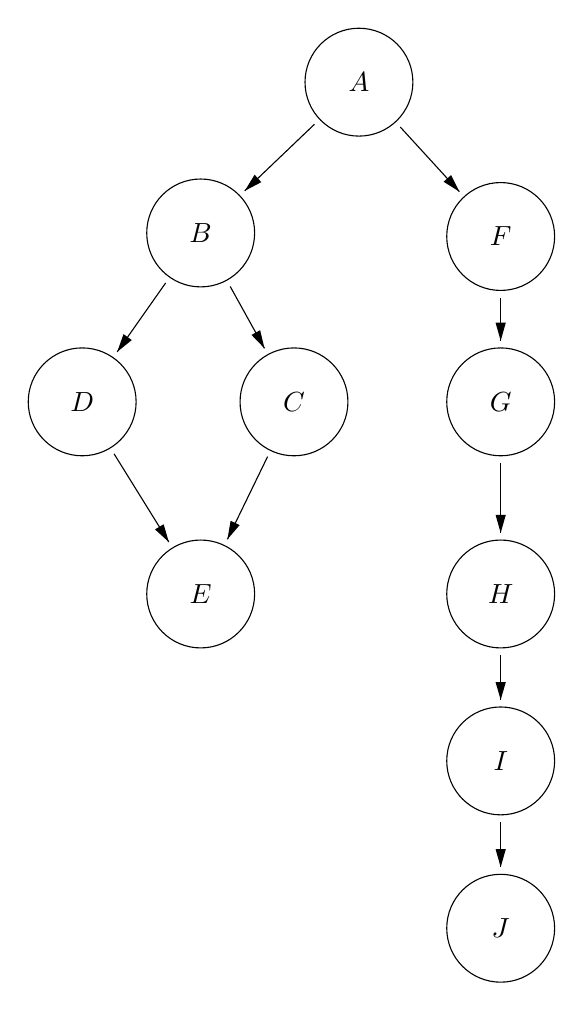
\begin{tikzpicture}[scale=0.5]
\draw (32.49, -2.33) circle (1.37);
\draw (32.49, -2.33) node { $A$};
\draw (28.47, -6.16) circle (1.37);
\draw (28.47, -6.16) node { $B$};
\draw (30.84, -10.45) circle (1.37);
\draw (30.84, -10.45) node { $C$};
\draw (25.46, -10.45) circle (1.37);
\draw (25.46, -10.45) node { $D$};
\draw (28.47, -15.33) circle (1.37);
\draw (28.47, -15.33) node { $E$};
\draw (36.09, -6.25) circle (1.37);
\draw (36.09, -6.25) node { $F$};
\draw (36.09, -10.45) circle (1.37);
\draw (36.09, -10.45) node { $G$};
\draw (36.09, -15.33) circle (1.37);
\draw (36.09, -15.33) node { $H$};
\draw (36.09, -19.57) circle (1.37);
\draw (36.09, -19.57) node { $I$};
\draw (36.09, -23.82) circle (1.37);
\draw (36.09, -23.82) node { $J$};
\draw (31.36, -3.40) -- (29.59, -5.09);
\fill (29.84,-4.68) -- (30.01,-4.87) -- (29.59,-5.09) -- cycle;
\draw (33.54, -3.47) -- (35.04, -5.11);
\fill (34.64,-4.86) -- (34.83,-4.69) -- (35.04,-5.11) -- cycle;
\draw (36.09, -7.80) -- (36.09, -8.90);
\fill (35.96,-8.44) -- (36.22,-8.44) -- (36.09,-8.90) -- cycle;
\draw (36.09, -12.00) -- (36.09, -13.78);
\fill (35.96,-13.32) -- (36.22,-13.32) -- (36.09,-13.78) -- cycle;
\draw (36.09, -16.88) -- (36.09, -18.02);
\fill (35.96,-17.57) -- (36.22,-17.57) -- (36.09,-18.02) -- cycle;
\draw (36.09, -21.13) -- (36.09, -22.27);
\fill (35.96,-21.81) -- (36.22,-21.81) -- (36.09,-22.27) -- cycle;
\draw (29.22, -7.52) -- (30.09, -9.09);
\fill (29.76,-8.75) -- (29.98,-8.63) -- (30.09,-9.09) -- cycle;
\draw (27.58, -7.43) -- (26.35, -9.18);
\fill (26.51,-8.73) -- (26.72,-8.88) -- (26.35,-9.18) -- cycle;
\draw (26.27, -11.77) -- (27.66, -14.01);
\fill (27.31,-13.69) -- (27.53,-13.56) -- (27.66,-14.01) -- cycle;
\draw (30.17, -11.84) -- (29.15, -13.94);
\fill (29.23,-13.47) -- (29.46,-13.58) -- (29.15,-13.94) -- cycle;
\end{tikzpicture}
\end{center}
\item Minimal element is because is the only one without arrows goind into it $A$, maximal element is $E$ because is the only one with 2 predecesors
\end{enumerate}
    \end{document}